\documentclass[11pt]{article}
\usepackage{times}
\usepackage{amsmath,amsthm,amssymb,setspace,enumitem,epsfig,titlesec,verbatim,color,array,eurosym,multirow}
\usepackage[sort&compress,comma,round]{natbib}
\usepackage[footnotesize,bf]{caption}
\usepackage[margin=2.5cm, includefoot, footskip=30pt]{geometry}
\usepackage{standalone}
\usepackage{tikz}
\usepackage{subcaption}
\usepackage{hyperref}
\usepackage{tabularx}
\usepackage{booktabs}
\usepackage{blkarray}
\usepackage[ruled,vlined]{algorithm2e}
\smallskip % Erlaubt kleine Abstaende zwischen Paragraphen, falls es dem Seitenlayout hilft
\renewcommand{\baselinestretch}{1.3}
\newcommand{\R}{\mathbb{R}}

\newcommand{\todo}[1]{\textcolor{blue}{#1}}

\def\alld{\texttt{ALLD}}
\def\tft{\texttt{TFT}}
\def\gtft{\texttt{GTFT}}
\def\esm{electronic supplementary material}

%% Adding shortcut commands to refer to our figures %%
\newcommand{\FigEvoProc}{{\bf Fig.~1}} 
\newcommand{\FigInvAnalysis}{{\bfFig.~2}} 
\newcommand{\FigResultsOverPara}{{\bf Fig.~3}}


\titleformat{\section}{\sffamily \fontsize{12}{14}\bfseries}{\thesection}{1em}{}
\titleformat{\subsection}{\sffamily
\fontsize{11.5}{11.5}\bfseries}{\thesubsection}{1em}{}

\usepackage{tikz}
\usetikzlibrary{arrows}

\tikzset{treenode/.style = {align=center, inner sep=0pt, text centered,
  font=\sffamily}, arn_n/.style = {treenode, circle, white,
  font=\sffamily\bfseries, draw=black, inner sep=-6pt, fill=black, text
  width=1.5em},% arbre rouge noir, noeud noir
  arn_r/.style = {treenode, circle, red, text width=1.5em, very thick, inner
    sep=4pt},% arbre rouge noir, noeud rouge
  arn_x/.style = {treenode, rectangle, draw=black, minimum width=0.5em, minimum
    height=0.5em}% arbre rouge noir, nil
}

\newtheoremstyle{plainCl1}% name
{9pt}%      Space above, empty = 'usual value'
{9pt}%      Space below
{\it}% 	   Body font
{}%         Indent amount (empty = no indent, \parindent = para indent)
{\bfseries}% Thm head font
{.}%        Punctuation after thm head
{0.2cm}% Space after thm head: \newline = linebreak
{}%         Thm head spec

\newtheoremstyle{plainCl2}% name
{9pt}%      Space above, empty = 'usual value'
{9pt}%      Space below
{\it}% 	   Body font
{}%         Indent amount (empty = no indent, \parindent = para indent)
{\bfseries}% Thm head font
{$'$.}%        Punctuation after thm head
{0.2cm}% Space after thm head: \newline = linebreak
{}%         Thm head spec


\theoremstyle{plainCl1}
\newtheorem{Claim}{Claim}
\newtheorem{Thm}{Theorem}
\newtheorem{Prop}{Proposition}
\newtheorem*{Lem}{Lemma}
\newtheorem{Cor}{Corollary}
\newtheorem*{Def}{Definition}

\theoremstyle{plainCl2}
\newtheorem{Claim2}{Claim}




\title{\bf  \sffamily \Large Evolution of reciprocity %among individuals\\ 
with limited payoff memory\\}
\date{}
\author{\parbox[c]{16cm}{\centering \onehalfspacing 
Nikoleta E. Glynatsi$^1$,  Alex McAvoy$^{2,3}$, Christian Hilbe$^1$\\
$^{\rm 1}$Max Planck Research Group on the Dynamics of Social Behavior,\\ Max Planck Institute for Evolutionary Biology, Pl\"{o}n, Germany \\
$^{\rm 2}$School of Data Science and Society, University of North Carolina at Chapel Hill,\\ Chapel Hill, NC 27599 \\
$^{\rm 3}$Department of Mathematics, University of North Carolina at Chapel Hill,\\ Chapel Hill, NC 27599}}

\begin{document}
\maketitle


\begin{abstract}
\noindent
Direct reciprocity can explain how cooperation emerges in repeated social interactions. 
According to this literature, individuals should naturally learn to adopt conditionally cooperative strategies, such as Tit-for-Tat. % if they expect to have further encounters with their interaction partner. 
Corresponding models have greatly facilitated our understanding of cooperation, yet they often make strong assumptions on how individuals remember and process information. 
For example, when strategies are updated through social learning, it is commonly assumed that individuals compare their respective average payoffs.  
This would require them to compute (or remember) their payoffs against all other population members.
Instead, herein, we introduce a theoretical framework to study the evolution of reciprocity when individuals learn based on their most recent experiences.
Even in the most extreme case that they only take into account their very last interaction, we find that cooperation can still evolve. 
However, such individuals adopt less generous strategies, and they tend to cooperate less often than in the classical setup with expected payoffs. 
Interestingly, once individuals remember the payoffs of two or three recent interactions, evolving cooperation rates quickly approach the classical limit. 
These findings contribute to a literature that explores which kind of cognitive capabilities are required for reciprocal cooperation. 
While our results suggest that some rudimentary form of payoff memory is necessary, it already suffices to remember a few interactions.\end{abstract}

~\\
{\it Keywords:} Evolution of cooperation; direct reciprocity; repeated prisoner's dilemma; social learning; evolutionary dynamics



\clearpage
\newpage


%%%%%%%%%
%%  INTRO  %%
%%%%%%%%%

\section{Introduction}

%% INTRO: General introduction to evolutionary game theory and cognitive constrains

Evolutionary game theory describes the dynamics of populations when an individual's fitness depends on the traits or strategies of other population members~\cite{hofbauer1998evolutionary, nowak:Nature:2004, hauert2005game}.  
This theory can be used to describe the dynamics of animal conflict~\citep{maynard-smith:Nature:1973}, cancer cells~\citep{Stein:PTRS:2023}, and of cooperation~\citep{nowak:Science:2006}. 
Respective models translate strategic interactions into games~\cite{smith1982evolution}. 
These games specify how individuals (players) interact, which strategies they can choose, and what fitness consequences (or payoffs) their strategies have. 
In addition, these models also specify the mode by which successful strategies spread over time. 
Models of biological evolution posit that individuals with a high fitness tend to produce more offspring; models of cultural evolution instead assume that such individuals are imitated more often. 
Although biological and cultural evolution are sometimes treated as equivalent, there can be important differences~\citep{Wu2015,Smolla:PTRS:2021}. 
For example, models of biological evolution do not require individuals to have any particular cognitive abilities.
Here, it is the evolutionary process itself that biases the population towards strategies with higher fitness. 
In contrast, in models of cultural evolution, individuals need to be aware of the different strategies present in the population, and they need to identify those strategies with a higher payoff. 
As a consequence, evolutionary outcomes may depend on how easily different behaviors can be learned~\citep{Chatterjee:JTB:2012}, and on how easy payoff comparisons are. 

%% INTRO: Literature on direct reciprocity and why social learning of strategies is hard

These difficulties -- to learn strategies by social imitation -- are particularly pronounced in models of direct reciprocity. 
This literature follows Trivers' insight that individuals have more of an incentive to cooperate in social dilemmas when they interact repeatedly~\citep{trivers1971evolution}. 
In repeated interactions, individuals can condition their future behavior on their past experiences with their interaction partner. 
They may use strategies such as Tit-for-Tat~\citep{rapoport:book:1965,axelrod1981evolution} or Generous Tit-for-Tat~\citep{molander:jcr:1985,Nowak1992tit} to preferentially cooperate with those partners who cooperated in the past. 
Such conditional strategies approximate human behavior fairly well~\citep{fischbacher:EconL:2001,Rand:TCS:2013,DalBo:AER:2019,Rossetti:ETH:2023} and they have also been documented in several other species~\citep{Carter:PRSB:2013,Schweinfurth:AnBehav:2019,Voelkl:PNAS:2015} -- although direct reciprocity is generally more difficult to demonstrate in animals~\citep{CluttonBrock:Nature:2009,Silk:CurrentBiology:2013,taborsky:CurrentBiology:2013}.
However, at the outset, it is not clear how easy it is to {\it learn} such strategies by social imitation. 
As one obstacle, individuals usually only observe other population members' actions (i.e., whether they cooperate or defect). 
These observations alone may not suffice to infer the underlying strategies (i.e., the contingent rules that determine whether to cooperate or defect in a given situation). 
As another obstacle, even if others' strategies are observable, individuals might find it difficult to identify which ones have the highest payoff. 
After all, the payoff of a strategy of direct reciprocity is not determined by the outcome of any single round.
Rather it is determined by how well this strategy fares over an entire sequence of rounds, against many different population members. 
In practice, such information might be both difficult to obtain and difficult to process. 

%% INTRO: Gap in the literature and what  question we wish to address. 

Most models of direct reciprocity abstract from these difficulties~\citep{brauchli:JTB:1999,brandt:JTB:2006,ohtsuki:JTB:2007b,szolnoki:pre:2009b,imhof2010stochastic,van-segbroeck:prl:2012,grujic:jtb:2012,Martinez2012,stewart:pnas:2013,pinheiro:PLoSCB:2014,stewart:games:2015,Baek2016,McAvoy:ProcA:2019,glynatsi:SCR:2020,Schmid:PlosCB:2022,Murase:SciRep:2022}. 
Instead they assume individuals can easily copy the strategies of others. 
Similarly, they assume that updating decisions are based on the strategies' average (or expected) payoffs, taking into account all rounds and interactions. 
These assumptions create a curious inconsistency in how models represent an individual's cognitive abilities. 
On the one hand, when playing the game, individuals are often assumed to have restricted memory. 
Respective studies typically assume that individuals make their decisions each round based on the outcome of the last round only~\citep[with only a few exceptions, see Refs.][]{Hauert1997,van-veelen:PNAS:2012,Stewart2016,Li:NatCS:2022,Murase:PLoSCompBio:2023a}. 
Yet when learning new strategies, individuals are assumed to remember (or compute) each others' precise average payoff across many rounds and many interaction partners. 
Herein, we wish to explore whether this latter assumption is actually necessary for the evolution of reciprocity through social imitation. 
We ask whether individuals can learn to adopt reciprocal strategies even when learning is based on payoff information from a limited number of rounds. 


%% INTRO: Basic description of our model and our findings 

To explore that question, we first consider two extreme scenarios. 
The first scenario corresponds to the usual modeling approach. 
Here, individuals update their strategies for a repeated prisoner's dilemma based on pairwise comparisons~\cite{traulsen2007pairwise}, taking into account their expected payoffs. 
We contrast this model with an alternative scenario where individuals update their strategies based on the very
last (one-shot) payoff they obtained. 
We find that individuals with limited payoff memory tend to adopt less generous strategies, yet moderate levels of cooperation can still evolve. 
Moreover, as we increase the individuals' payoff memory to include the last two or three one-shot payoffs, cooperation rates quickly approach the rates observed in the classical baseline case. 
Overall, these findings suggest that while memory is important, already minimal payoff information may suffice for the evolution of direct reciprocity based on social learning. 
They also suggest that the classical model of reciprocity (based on expected payoffs) can often be interpreted as a useful approximation to more realistic models that include cognitive constraints. 



\section{Model and Methods}\label{section:model}

%% MODEL: Basic intro

To explore the impact of limited payoff memory, we adapt existing models of the evolution of direct reciprocity through social learning. 
These models consider the dynamics on two different time scales. 
The short time scale describes the game dynamics. 
Here, individuals with fixed strategies are randomly matched to interact with each other in a series of repeated social dilemmas. 
The long time scale describes the evolutionary dynamics. 
Here, individuals can update their strategies based on the payoffs they yield. 
In the following, we describe the basic setup of our model; all details and derivations are described in the \esm.\\

%% MODEL: (Repeated) donation game

\noindent
{\bf Description of the game dynamics.} For our model, we consider a well-mixed population consisting of $N$~players.
Players are randomly matched in pairs to participate in a repeated donation game~\citep{sigmund2010calculus}.
Each round, players can either cooperate (\(C\)) or defect (\(D\)). 
By cooperating, a player provides a benefit \(b\) to the other player at their cost \(c\), with \(0 \!<\! c \!<\! b\). 
Thus, the players' payoffs in a single round are given by the matrix

\begin{equation}
    \begin{blockarray}{ccc}
        & \text{cooperate} & \text{defect} \\
        \begin{block}{c(cc)}
            \text{cooperate} & b - c & -c \\
            \text{defect} & b & 0 \\
        \end{block}
    \end{blockarray}.
\end{equation}
In particular, payoffs take the form of a prisoner's dilemma.
Mutual cooperation yields a better payoff than mutual defection ($b\!-\!c\!>\!0$), but each player individually prefers to defect independent of the co-player's action ($b\!>\!b\!-\!c$ and $0\!>\!-c$). 
To incorporate that individuals interact repeatedly, we assume that after each round, there is a constant continuation probability $\delta$ of interacting for another round. 
For $\delta\!=\!0$, we recover the case of a conventional (one-shot) prisoner's dilemma. 
Here, mutual defection is the only equilibrium. 
As $\delta$ increases, the game turns into a repeated game. As a result, additional equilibria emerge, with some of them allowing for full cooperation~\citep{friedman:RES:1971,Akin:chapter:2016,hilbe:GEB:2015,stewart:pnas:2014}. 


%% MODEL: Reactive strategies

In a one-shot donation game, players can only choose among two strategies (either cooperate or defect).
In the repeated game, strategies can become arbitrarily complex. 
Here, strategies are contingent rules, telling players what to do depending on the outcome of all their previous interactions. 
For simplicity, in the following we assume individuals use {\it reactive strategies}~\citep{Nowak1992tit}. 
A reactive strategy only depends on the other player's action in the previous round. 
As a consequence, reactive strategies can be written as a three-dimensional tuple \(\mathbf{s}=(y, p,q)\). 
The first entry \(y\) is the probability that the player opens with cooperation in the first round. 
The two other entries are the probabilities that the player cooperates in all subsequent rounds, depending on whether the co-player cooperated~($p$) or defected~($q$) in the previous round. 
The set of reactive strategies is simple enough to allow for an explicit mathematical treatment~\citep{hofbauer1998evolutionary}. 
Yet it is rich enough to capture several important strategies of repeated games. 
For example, it contains \alld{} $=\!(0,0,0)$, the strategy that always defects. 
Similarly, it contains Tit-for-Tat, \tft{} $=\!(1,1,0)$, the strategy that copies the co-player's previous action (and that cooperates in the first round). 

In the short run, the players' strategies are taken to be fixed.
Players use their strategies to decide whether to cooperate with any given interaction partner. 
In the long run, however, the players' strategies may change depending on the payoffs they yield, as we describe in the following.\\
 
 %% MODEL: Pairwise comparison process

\noindent
{\bf Description of the evolutionary dynamics.}
Herein, we assume population members update their strategies based on social learning. 
To model these strategy updates, we consider a pairwise comparison process~\citep{traulsen2007pairwise}. 
This process assumes that at regular time intervals, one population member is randomly selected, and given the chance to update its strategy.
We refer to this player as the `learner'. 
With probability $\mu$ (reflecting a mutation rate), the learner simply adopts a random strategy (with all reactive strategies having the same probability to be chosen). 
With the converse probability $1\!-\!\mu$, the learner randomly picks a `role model' from the population. 
The learner then compares its own payoff $\pi_L$ from the repeated game stage to the payoff $\pi_R$ of the role model. 
The learner adopts the role model's strategy with a probability \(\rho\) described by a Fermi function~\citep{blume:GEB:1995,szabo:PRE:1998}, 
\begin{equation} \label{Eq:rho}
    \rho(\pi_{L}, \pi_{R}) = \frac{1}{1\!+\! e^{- \!\beta (\pi_{R}- \pi_{L})}}.
\end{equation}
Here, the selection strength $\beta\!\ge\!0$ is a parameter that indicates how sensitive players are to payoff differences. 
For $\beta\!=\!0$, any payoff differences are irrelevant, and the learner simply adopts the role model's strategy with probability one half. As the selection strength~$\beta$ increases, players are increasingly biased to update only if the role model has the higher payoff. 
In either case, we assume that the role model's strategy can be identified.
That is, if the learner decides to imitate the role model's strategy, the learner copies it exactly, as assumed in most previous work on direct reciprocity. 

%% MODEL: Perfect vs limited payoff memory

We deviate from previous models in how we interpret the payoffs $\pi_L$ and $\pi_R$, which form the basis of the pairwise comparisons in Eq.~\eqref{Eq:rho}. 
In previous work, these payoffs are taken to be the respective players' expected payoffs. 
We interpret this setup as a model with perfect payoff memory. 
In this setup, the payoffs  $\pi_L$ and $\pi_R$ represent an average over all possible repeated games the two individuals could have played with all population members. 
The use of expected payoffs is mathematically convenient, because explicit formulas for the players' expected payoffs are available~\citep{hofbauer1998evolutionary}.
Herein, we compare this model to a model with limited payoff memory. 
In that model, the players' payoffs $\pi_L$ and $\pi_R$ are taken to be the payoffs that each player received in the last round of the last repeated game they interacted in (see \FigEvoProc\textbf{a}). 
This assumption could reflect, for example, a strong recency bias in how individuals evaluate their payoffs.  
In addition to this extreme case of limited payoff memory, later on we also explore cases in which players take into account the outcome of two, three, or four recent rounds. 

Both in the case of perfect and limited memory, we iterate this elementary pairwise comparison process for many time steps. 
This gives rise to a stochastic process that describes which strategies players adopt over time. 
We explore the dynamics of this process with computer simulations.
For the results presented in the following, we assume that mutations are rare (\(\mu\!\rightarrow\! 0\)). 
This assumption is fairly common in evolutionary game theory, because it makes computations more efficient~\citep{fudenberg:JET:2006,wu:JMB:2012,mcavoy:jet:2015}, and because the results can be interpreted more easily.  
However, in Section~9 of the \esm{} we show that our main result holds continue to hold for strictly positive mutation rates.



\section{Results}

\noindent
{\bf Stability of cooperative populations.}
To get some intuition for the differences between perfect and limited payoff memory, we first analyze when cooperation is stable in either scenario.
To this end, we consider a resident population in which all players but one adopt a strategy of Generous Tit-for-Tat, \gtft{} $=\!(1,1,q)$. 
The remaining mutant player adopts \alld. 
We say {\it cooperation is stochastically stable} if the single mutant is more likely to imitate the residents than vice versa. 
For simplicity, we consider a large population~($N\!\rightarrow\!\infty$) and strong selection~($\beta\!\rightarrow\!\infty$).
More general results are derived in the \esm. 

In the case of perfect payoff memory, it is straightforward to compute each player's expected payoff. 
Because the population mostly consists of residents, and because residents mutually cooperate with each other, their payoff is $\pi_\gtft = b\!-\!c$. 
The mutant only interacts with residents, and hence receives a benefit in the first round, and in every subsequent round with probability $q$. 
As a result, the mutant's expected payoff is $\pi_\alld \!=\! (1\!-\!\delta\!+\!\delta q)b$. 
For perfect payoff memory, the requirement for cooperation to be stochastically stable reduces to the condition $\pi_\gtft > \pi_\alld$. 
This yields
\begin{equation} \label{Eq:PerfectMemory}
q < 1\!-\!\frac{c}{\delta  b}.
\end{equation}
In particular, we recover that $q\!=\!1-c/(\delta b)$ is the maximum generosity that cooperators should have~\citep{molander:jcr:1985,Nowak1992tit}. 
Because $q$ needs to be non-negative, we also conclude that cooperation can only be stable if $\delta \!>\! c/b$.
Again, this condition for the feasibility of direct reciprocity is the condition found in the literature~\citep{nowak:Science:2006}.

The logic of the case with limited payoff memory is somewhat different. 
Here we need to compute how likely each player obtains one of the four possible payoffs $\{b\!-\!c, -c, b, 0\}$ in their last interaction. 
Because residents almost always interact with other residents, their last one-shot payoff is $\pi_\gtft = b\!-\!c$ with a probability approaching one. 
For the defecting mutant, there are two possibilities. 
({\it i})~ If the mutant's co-player happens to cooperate in the last round, the mutant receives a payoff of $\pi_\alld\!=\!b$.
This occurs with probability $1\!-\!\delta\!+\!\delta q$. 
({\it ii})~If the co-player defects in the last round, the mutant receives $\pi_\alld=\!0$. 
This case occurs with probability $\delta(1\!-\!q)$.
Because $b\!-\!c\!<\!b$, we conclude that  in the first case, residents tend to imitate the mutant. 
Because $b\!-\!c\!>\!0$, in the second case mutants tend to imitate the resident. 
Cooperation is thus stochastically stable if the first case is less likely than the second. 
This yields the condition
\begin{equation}
q < 1\!-\!\frac{1}{2 \delta}.
\end{equation}
Interestingly, this condition no longer depends on the exact payoff values $c$ and $b$ (this happens because selection is strong, such that only the payoff ordering $b\!>\!c\!>\!0$ matters). In particular, because $q$ is non-negative, this condition can only be satisfied if $\delta\!>\!1/2$. 

By comparing the two cases, we find that payoff memory affects which cooperative strategies are viable. 
With perfect memory, the maximum generosity $q$ needs to satisfy Eq.~\eqref{Eq:PerfectMemory}.
In particular, this generosity can become arbitrarily large, if only the game's benefit-to-cost ratio~$b/c$ and the continuation probability~$\delta$ are sufficiently large. 
In contrast, with limited payoff memory, the maximum generosity is bounded by one half, and it is independent of the benefit-to-cost ratio. 
To explore whether we indeed observe these patterns in evolving populations, we turn to simulations.\\

\noindent
{\bf Evolutionary dynamics with perfect and limited payoff memory.}
To assess the impact of updating payoffs, we simulate the evolutionary process,
recording the strategies adopted by players over time based on perfect and
limited payoff memory. We performed two separate runs for each approach varying
the value of benefit \(b\).
Figure~\ref{fig:expected_and_stochastic_for_donation} depicts the evolving
conditional cooperation probabilities $p$ and $q$ (note that we omit the opening
move \(y\), as the discount factor \(\delta\) is relatively high). The figure
suggests that when updating is based on perfect payoff memory players tend to be
more generous and more cooperative.

Specifically, we observe that the resident population comprises either defectors
or conditional cooperators \((1, q)\). The generosity level \(q\) adopted by the
resident population depends on whether a defecting strategy can invade.
Supplementary Information Section 2 and 3 show that in the perfect payoff memory
framework, conditional cooperators of the form \((1, q < \frac{c}{b})\) can
arise, however, in the case of limited payoff memory, only conditional
cooperators of \((1, q < \frac{1}{2})\) can avoid invasion. 
The $q$-values of the resident strategies are generally higher in classical
case, indicating that players are more likely to forgive a defection if their fitness
depends on interacting with every member of the population. This effect becomes
more pronounced as the benefit value increases, as the perfect memory condition
on the left-hand side increases, while in the limited memory case, it remains at
\(q \approx \frac{1}{2}\).

Higher $q$ values lead to a more cooperative population. We compute the average
cooperation rate for each simulation, which is the average cooperation rate
within the resident population. In the case of perfect payoff memory, the
average cooperation rate is consistently higher than that of the last round
payoffs.

We further investigate the impact of benefit and selection strength on
generosity $q$ and the cooperation rate, as shown in Figure~\ref{fig:cooperation_rate_over_benefit_and_beta}.
According to Figure~\ref{fig:cooperation_rate_over_benefit_and_beta}\textbf{A},
perfect memory consistently results in a higher cooperation rate, which
increases with increasing benefit. On the other hand, the cooperation rate
remains approximately 50\% for limited payoff memory once \(b = 5\).
From Figure~\ref{fig:cooperation_rate_over_benefit_and_beta}\textbf{B}
we observe that for weak selection, \(\beta < 1\), the two methods yield similar
results, however, as \(\beta\) increases there is variation in the evolving
populations. In the case of expected payoffs the resident populations become
more cooperative, whereas in the case of limited payoff memory, the resident
populations become more defective.

The limited payoff memory framework can be expanded by enabling individuals to
observe a greater number of rounds, interact with a larger number of members, or
both (refer to Supplementary Information Sections 4-6). To gain further insight
into the impact of limited payoff memory, we explore the scenarios of updating
based on the last round with two members of the population, the last two rounds
with another member of the population, and the last two rounds with two members
of the population. To analyze the effects of this framework, we conduct
numerical simulations using various fitness methods. The cooperation rates for
low and high benefits are presented in Figure~\ref{fig:cooperation_rate_all_updating_payoffs}.

We observe a significant rise in the cooperation rate with the introduction of
slightly more information. Specifically, in scenarios involving two rounds or
two interactions, the cooperation rates are almost identical. For a large
population and a high continuation probability ($\delta$), the conditional
cooperators that are adopted by the resident population in these scenarios take
on the same form \((1, q < \frac{\sqrt{2}}{2})\). When considering both sets
of information (i.e., two rounds and two interactions), cooperation rates
experience a greater increase, yet still remain lower compared to the classical
scenario.


\section{Conclusions}\label{section:conclusions}

Cooperation can be seen as odd, why is it that we choose to help others at a
personal cost? In spite of all the selfish genes', animal and human communities
show signs of altruism and cooperation~\cite{milinski1987tit, kerr2002local,
carter2020development}. Evolutionary game theoretical models have helped us
shape our understanding of the evolution of cooperation. In fact, the evolution
of cooperation constitutes such a major focus of the field that evolutionary
game theory seems to be reduced to the evolution of
cooperation~\cite{Traulsen:PhilTrans:2022}. 

Evolutionary models in the past often feature a curious inconsistency. While
these models depict how individuals make decisions in each round by assuming
that they only retain memory of the previous round, they also assume that
individuals possess a perfect memory when it comes to updating their strategies
over time. To be precise, individuals are assumed to remember all of their past
interactions and each interaction's outcome when updating strategies.

Here, we investigate the robustness of cooperation as models deviate
from the assumption of perfect memory. While prior research has investigated the
impact of constraining individuals' interactions, we take into account the
limitation of not only interactions but also the information available for each
outcome. Additionally, prior studies have only allowed for the adoption of
simple strategies such as always cooperating or always defecting. In contrast,
we enable the use of more intricate strategies where players can utilize the
previous play of their co-player to make decisions.

In our framework, players update their strategies based on a combination of
interactions and outcomes. The initial scenario we examined involved using one
piece of information: the last round of one interaction. The outcomes suggest
that cooperation faces difficulties in developing when the updating stage
utilizes minimal social information. This effect is compounded as the benefit
and strength of selection are independently increased. The findings indicate
that cooperative players benefit from the ability to engage with all members of
the population.

Furthermore, we investigated scenarios where the final two rounds, or the last
two instances of interaction, were taken into account. We observed a
statistically significant rise in the frequency of cooperative behavior. For a
sizable population and a high likelihood of continued interactions, the two
cases yield the same result as the overall payoff is influenced by two possible
outcomes. Notably, the scenario involving two rounds and two interactions
yielded the highest cooperation rate among all the novel methodologies that we
tested.\\
% A nice sentence missing here.



%%%%%%%%%%%
%% END NOTES %%
%%%%%%%%%%%

\begin{comment}

\noindent
{\bf Ethics.}
This work is purely theoretical and did not require ethical approval from a human subject or animal welfare committee.\\

\noindent
{\bf Data accessibility.}
All data and code used in this manuscript are openly available at https://github.com/Nikoleta-v3/pd-with-stochastic-payoffs \todo{(Correct?)}.\\

\noindent
{\bf Declaration of AI use.}
We have not used AI-assisted technologies in creating this article.\\

\noindent
{\bf Authors' contributions.}
N.G.: conceptualization, formal analysis, investigation, methodology, visualization, writing - original draft, writing -- review and editing; 
A.M.: conceptualization, formal analysis, methodology, writing -- review and editing; 
C.H.: conceptualization, formal analysis, methodology, writing -- review and editing.\\

\noindent
{\bf Conflict of interest declaration.}
We declare we have no competing interests.\\

\noindent
{\bf Funding.}
N.G. and C.H. acknowledge generous support by the European Research Council Starting Grant 850529:
E-DIRECT, and by the Max Planck Society.\\
\end{comment}



{
{\setlength{\bibsep}{0\baselineskip}\small
\bibliographystyle{naturemag}
\bibliography{bibliography.bib}
}

\clearpage
\newpage

\begin{figure}[!htbp]
    \centering
    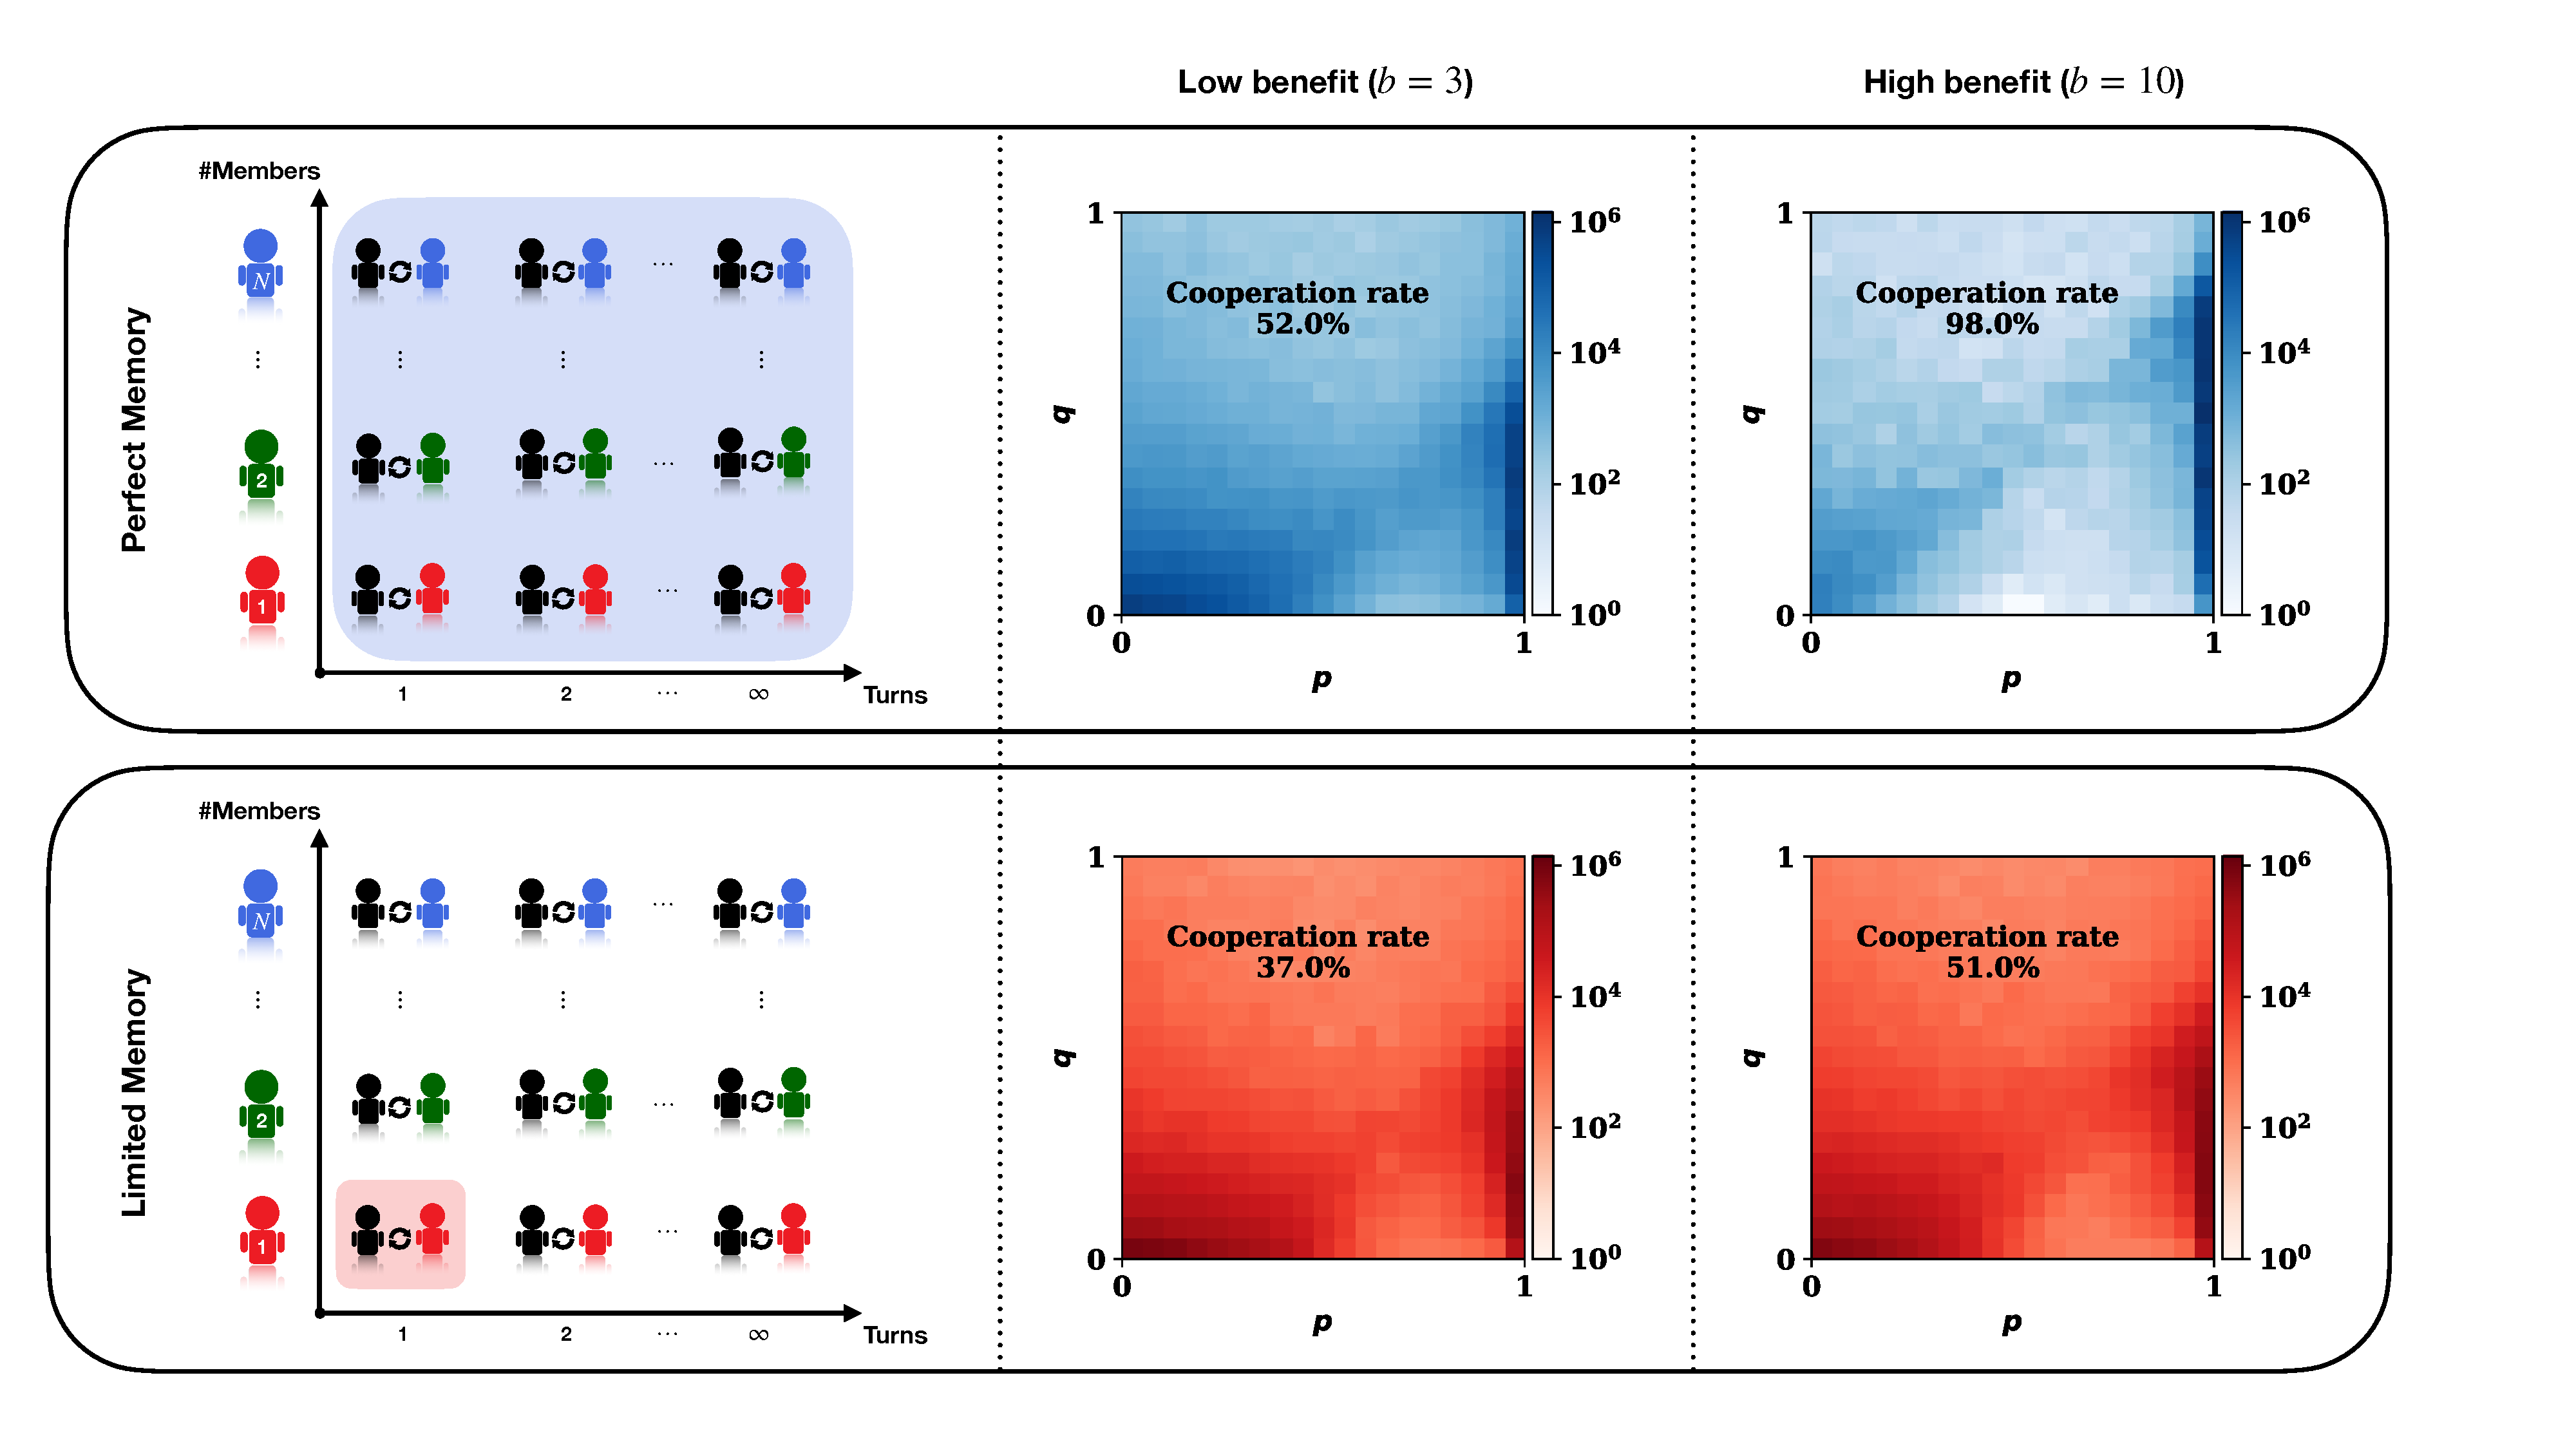
\includegraphics[width=\textwidth]{static/donation_expected_last_round_summary_results.pdf}
    \caption{{\bf Evolutionary dynamics under perfect and limited payoff memory.}
    ({\bf Schematic illustrations}) On the left panels we show schematic
    illustrations of the perfect memory and the limited memory cases. The shaded
    background denotes the game phase information that an individual considers
    when updating strategies. In the case of perfect payoff memory the entire region is
    shaded and in the case of limited payoff memory only one turn with a single member
    of the population. ({\bf Simulations}) We have run four simulations of the
    pairwise comparison process for $T\!=\!10^7$ time steps. For each time step
    of the process
    we record the current resident population ($y,p,q$). Since
    simulations are run for a relatively high continuation probability of
    $\delta\!=\!0.999$, we do not report the players' initial cooperation
    probability $y$. The plots show how often the resident population chooses
    each combination ($p,q$) of conditional cooperation probabilities in the
    subsequent rounds. We also report the evolved cooperation rate which is
    calculated as the average cooperation rate within the resident population.
    ({\bf Perfect Memory}) In the case of low benefit the resident population
    either consists of defectors (with $p\!\approx\!q\!\approx\!0$) or of
    conditional cooperators. Conditional cooperators, or otherwise known as
    generous tit for tat, are a set of strategies that always cooperate
    following a cooperation ($p\!\approx\!1\!$) and cooperate with a probability
    $q$ given that the co-player has defected. $q$ denotes the generosity of a
    player. The resident population applies a conditional cooperator strategy
    for which $q\!\le\!1\!-\!c/b\!=\!0.67$. 
    In the case of high benefit the population mainly consists of conditional
    cooperators of the form ($p\!\approx\!1\!, q\!\le\!1\!-\!1/10\!=\!0.9$). In
    the Supplementary Information Section 2 we show that a conditional
    cooperator needs to be of the form ($p\!\approx\!1\!, q\!\le\!1\!-\!c/b$) to
    not be invaded by defecting strategies. A higher generosity in the
    population results in a higher average cooperation rate. The average
    cooperation rate increases from 52\% for \(b=3\) to 98\% for \(b=10\). ({\bf
    Limited Memory}) When players update their strategies based on their
    realized payoffs in the last round, there are two different predominant
    behaviors regardless of the benefit value. The resident population either
    consists of defectors (with $p\!\approx\!q\!\approx\!0$) or of conditional
    cooperators. The maximum level of $q$, consistent with stable cooperation, is
    somewhat smaller compared to the perfect memory setting.
    Namely, in the Supplementary Information Section 3 we show that
    regardless of the value of benefit a conditional cooperator need to be of
    the form $q\!<\!\frac{1}{2}$ to not be invaded by defectors.
    The evolved cooperation
    rate only slightly increases from 37\% ($b=3$) to 51\% ($b=10$). Parameters: $N\!=\!100$,
    $c\!=\!1$, $\beta\!=\!1$, $\delta\!=\!0.999$.}
    \label{fig:expected_and_stochastic_for_donation}
\end{figure}

\begin{figure}[!htbp]
    \centering
    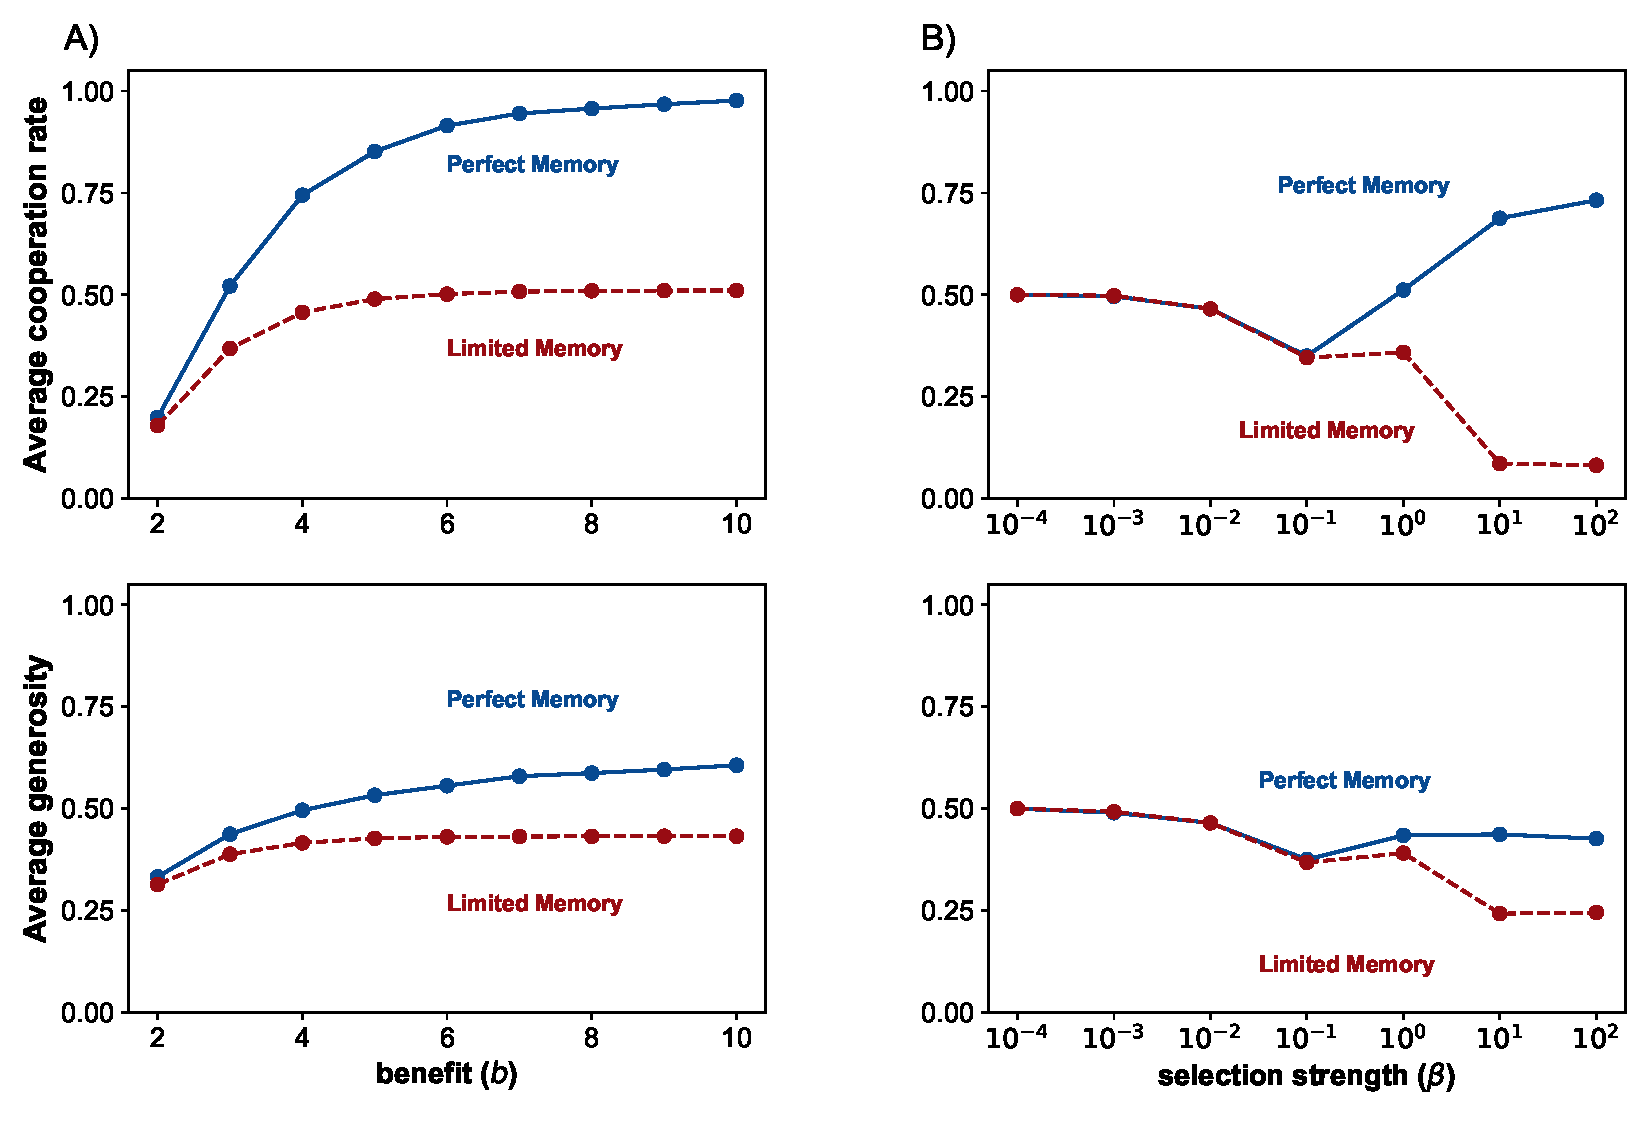
\includegraphics[width=.75\textwidth]{static/cooperation_rate_over_b_and_beta.pdf}
    \caption{{\bf The evolution of cooperation and generosity for different
    values of benefit (A) and strength of selection (B).} We report the average
    cooperation and the average reciprocity. The average cooperation rate is the
    average cooperation rate within the resident population. For the average
    reciprocity we select the residents that have a $p \approx 1$ and we take
    the average of their cooperation probability $q$. ({\bf A}) We vary the
    benefit of cooperation $b$. In all cases, perfect memory updating payoffs
    appear to overestimate the average cooperation rate the population achieves.
    As expected in the case of limited memory the average generosity over the
    different values of benefit remains the same ($q \approx 0.5$), and as a
    result so does the average cooperation. ({\bf B}) We vary the selection
    strength $\beta$. For weak selection, \(\beta < 1\), the two methods yield
    similar results. However, as \(\beta\) increases in the case of limited
    memory payoffs the resident populations become more defective. Note that
    in the case of perfect payoff memory we see an increase in the cooperation
    rate even though the generosity remains stable. That is because the
    generosity does remain the same, however, now cooperative strategies remain
    fixed as the resident strategy for longer.
    Unless
    explicitly varied, the parameters of the simulation are $N\!=\!100$,
    $b\!=\!3$, $c\!=\!1$, $\beta\!=\!1$, $\delta\!=\!0.99$. Simulations are run
    for $T\!=\!5\times 10^7$ time steps for each parameter
    combination.}\label{fig:cooperation_rate_over_benefit_and_beta}
\end{figure}


\begin{figure}[!htbp]
  \centering
  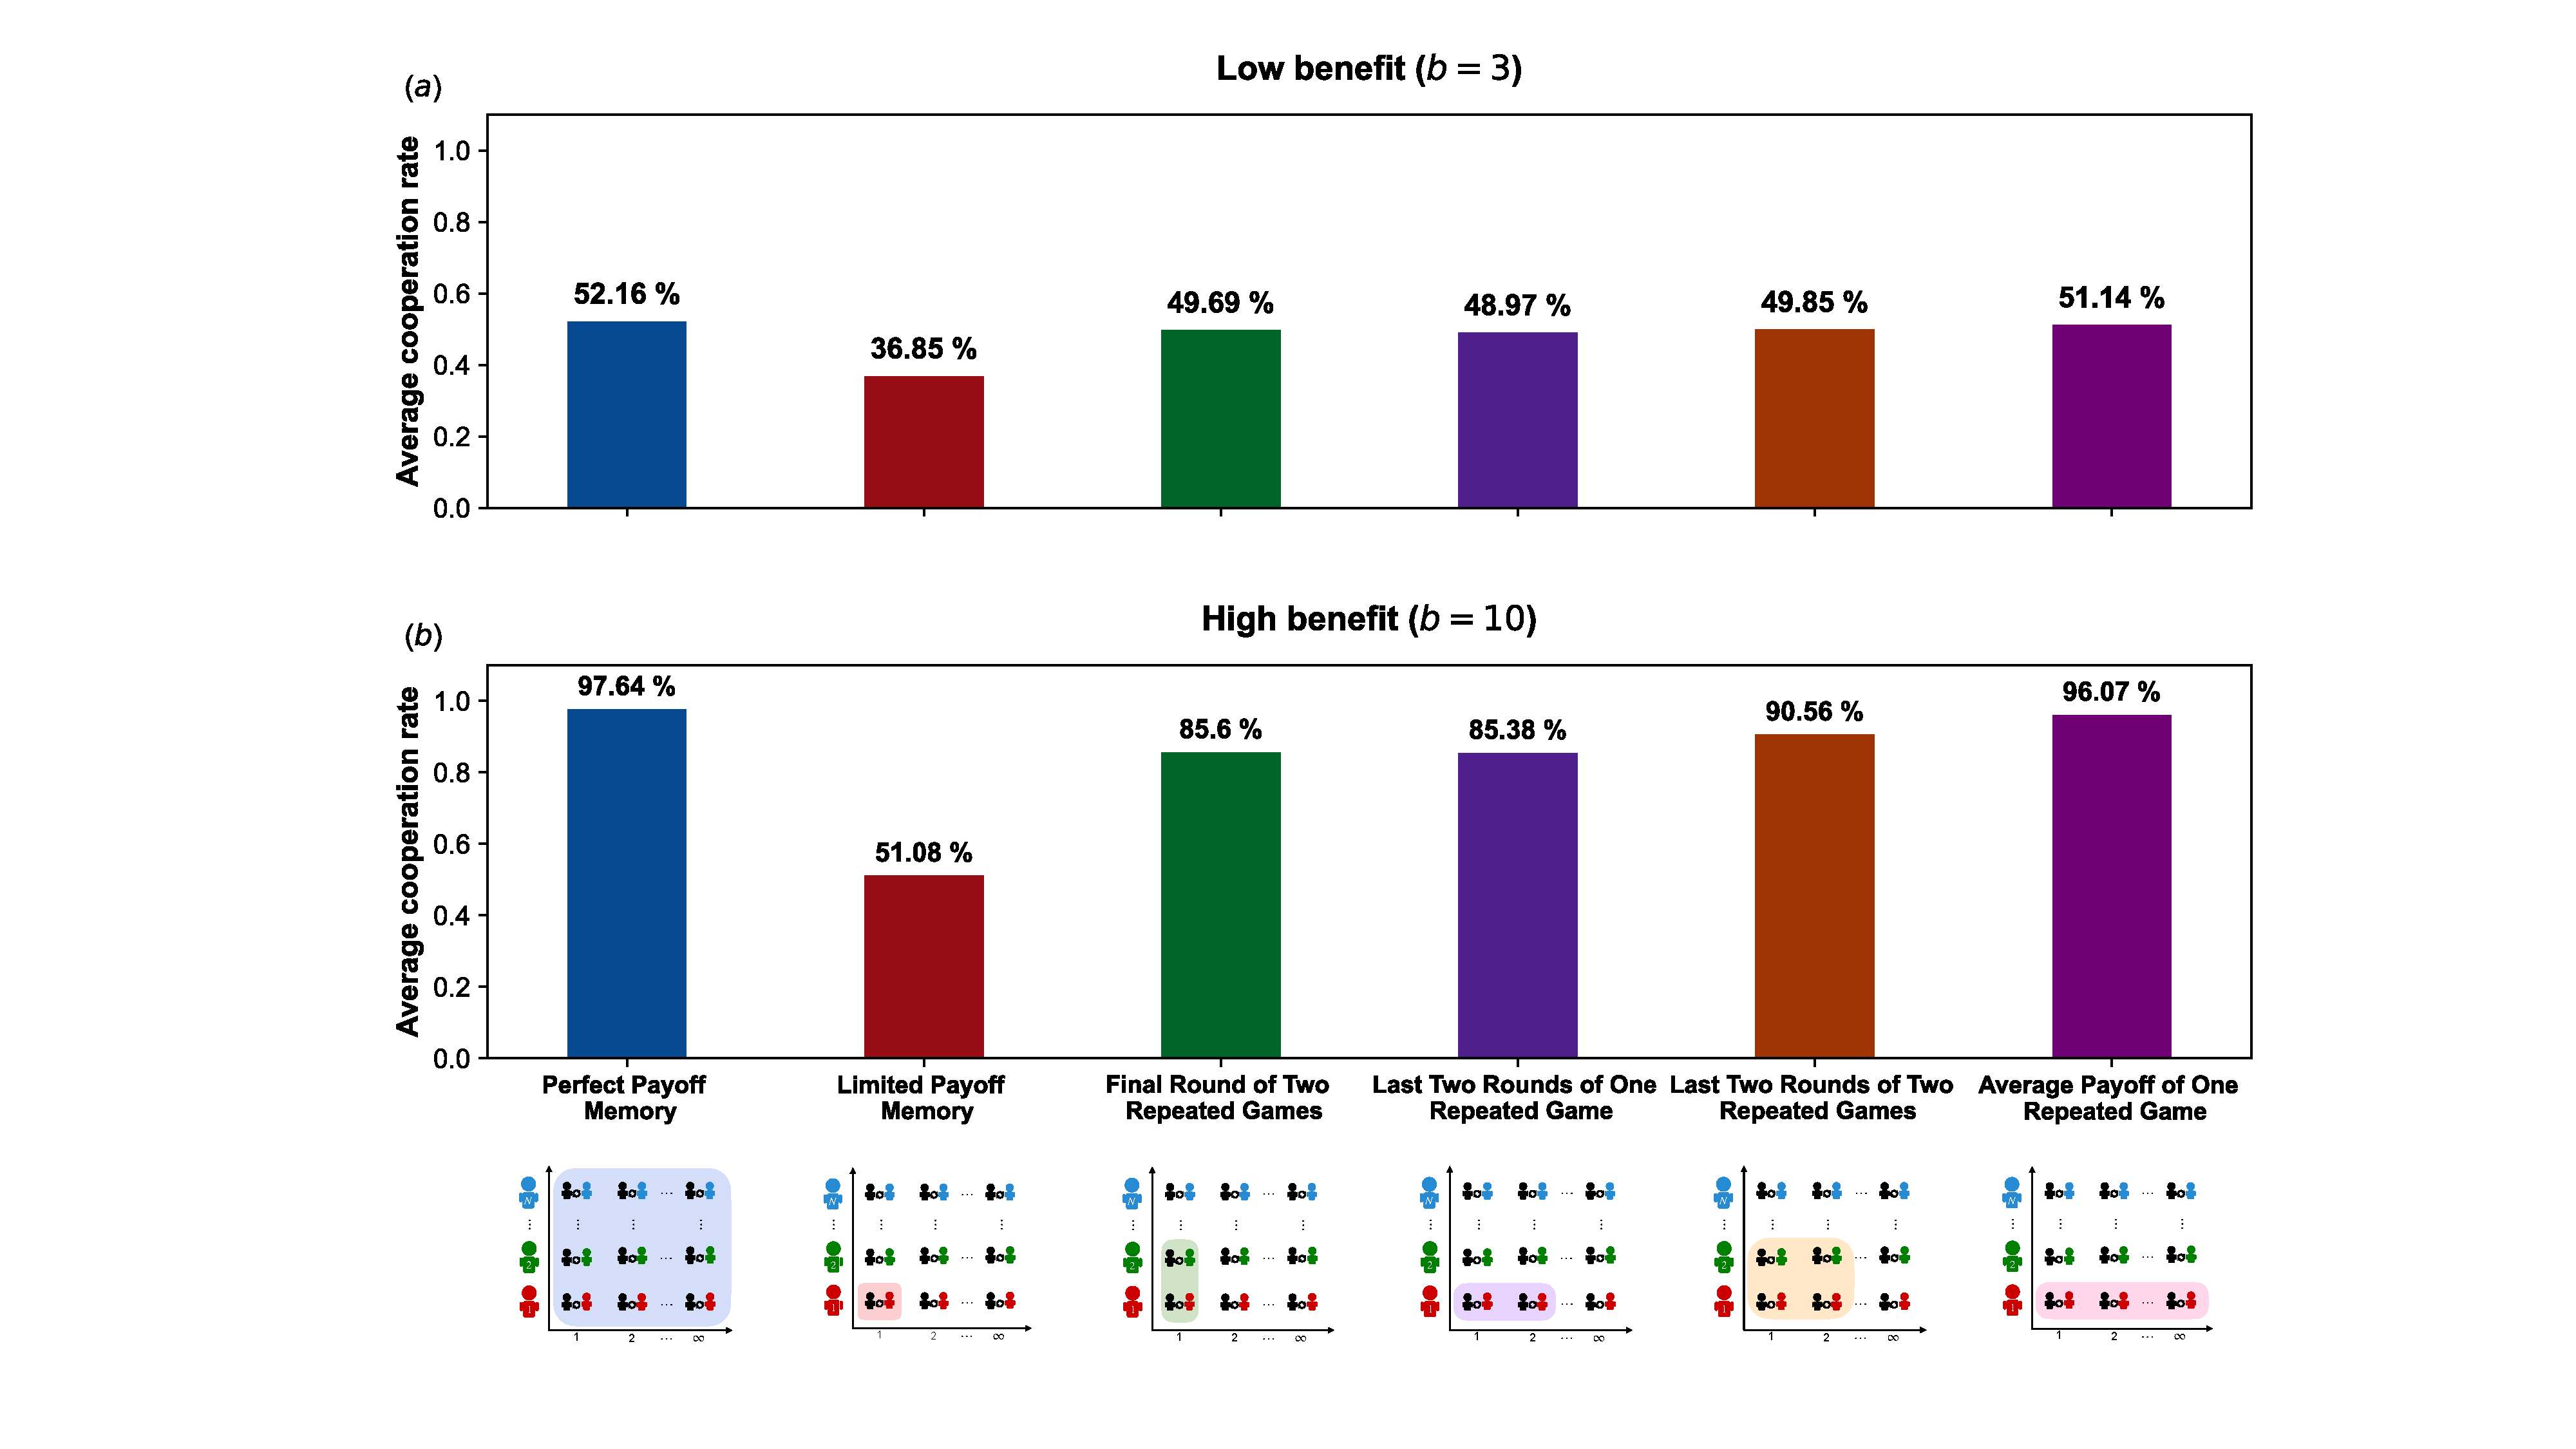
\includegraphics[width=\textwidth]{static/more_memory_summary_results.pdf}
  \caption{{\bf Average cooperation rates for different updating payoffs.}
  From left to right, we present result on the following updating payoffs cases;
  (a) the expected payoffs (perfect memory), (b) the last round payoff from one
  interaction (limited memory), (c) the last round payoff from two interactions,
  (d) the last two rounds payoffs from one interaction, (e) the last two rounds
  payoffs from two interactions. For the updating payoffs (c) and (d) we have
  carried out an analysis which has shown that conditional cooperators should
  adopt a \(q\) value smaller than $\frac{\delta - 1 +
  \frac{\sqrt{2}}{2}}{\delta}$ and $\frac{\delta + \sqrt{\delta^{2} + 1} - 1}{2 \delta}$
  respectively. Note that as \(\delta
  \rightarrow 1\) both right hand sides tend to \(\frac{\sqrt{2}}{2}\).
  Regardless the cooperation rate between for case (c) is slightly higher.
  In case (d) the cooperation rate is the second highest hinting that as we
  allow for more information the closer we move to the perfect payoff memory.
  We performed four pairwise non parametric tests (Mann-Whitney U) to compare
  the cooperation distributions of the residents in case (b) to
  cases (a), (c), (d), (e). In all four tests we reject the null hypothesis
  with \(\alpha=0.05\) and \(p \approx 0\). Thus, there is significant
  difference between the cooperation rates.
  Unless explicitly varied, the parameters of the simulation are
  $N\!=\!100$, $b\!=\!3$, $c\!=\!1$, $\beta\!=\!1$, $\delta\!=\!0.99$.
  Simulations are run for $T\!=\!5\times 10^7$ time steps for each parameter
  combination.}\label{fig:cooperation_rate_all_updating_payoffs}
\end{figure}



\end{document}





%% SOME ADDITIONAL TEXT BITS %%


% repeated game markov chain
given that the opponent cooperated and defected equivalently. The play between a
pair of reactive strategies $s_1 = (y_1, p_1, q_1)$ and $s_2 = (y_2, p_2, q_2)$
can be model as a Markov process with the transition matrix \(M\)~\cite{nowak:APC:1989},

\begin{equation}\label{eq:transition_matrix}
  M = \left[\begin{matrix} p_{1} p_{2} & p_{1} \left(1 - p_{2}\right) & p_{2} \left(1 - p_{1}\right) & \left(1 - p_{1}\right) \left(1 - p_{2}\right)\\
    p_{2} q_{1} & q_{1} \left(1 - p_{2}\right) & p_{2} \left(1 - q_{1}\right) & \left(1 - p_{2}\right) \left(1 - q_{1}\right)\\
    p_{1} q_{2} & p_{1} \left(1 - q_{2}\right) & q_{2} \left(1 - p_{1}\right) & \left(1 - p_{1}\right) \left(1 - q_{2}\right)\\
    q_{1} q_{2} & q_{1} \left(1 - q_{2}\right) & q_{2} \left(1 - q_{1}\right) & \left(1 - q_{1}\right) \left(1 - q_{2}\right)\end{matrix}\right]
\end{equation}

and the stationary vector \(\mathbf{v}(s_1,s_2)\)
which is the solution to \(\mathbf{v}(s_1,s_2) \times M 
= \mathbf{v}(s_1,s_2)\).




% pairwise comparison fixation probability

In fact, so rare that only two different strategies can be
present in the population at any given time. However, in the Supplementary Information
Section 9 we show that the main result holds for \(\mu \neq 0\).
The case of low mutation is vastly adopted because it allows us to explicitly
calculate the fixation probability of a newly introduced mutant. More specifically,
at each step
one individual adopts a mutant strategy randomly selected from the set of
feasible strategies. The fixation probability \(\phi_{M}\) of the mutant
strategy can be calculated explicitly as,

\begin{equation}\label{eq:appendix_fixation_probability}
    \varphi_{M} = \frac{1}{1+\sum\limits_{i=1}^{N-1}\prod\limits_k^i \frac{\lambda^-_k}{\lambda^+_k}},
\end{equation}

where \(k\) is the number of
mutants and \(\lambda^-_k, \lambda^+_k\) are the probabilities that the number of
mutants decreases and increases respectively.
Depending on the fixation probability \(\phi_{M}\) the mutant either
fixes (becomes the new resident) or goes extinct. Regardless, in the next elementary
time step another mutant strategy is introduced to the population. We iterate
this elementary population updating process for a large number of mutant
strategies and we record the resident strategies at each time step. The
probabilities \(\lambda^-_k \text{ and } \lambda^+_k\) depend on the fitness
of the mutant and the resident strategies. In the next section we
present how fitness is calculated in the cases of perfect and limited payoff memory.




% Explicit formulas for the transition probabilities for perfect and limited memory

\subsection{Fitness based on Perfect and Limited Payoff Memory}

In the perfect payoff memory case an individual updates based on the average payoff
against each other member of the population, otherwise known as expected payoffs. 
The payoff of a reactive strategy \(s_1\) against the reactive strategy \(s_2\)
in an infinitely repeated game ($\delta \rightarrow 1$) is explicitly
calculated as,

\[\langle\mathbf{v}(s_1,s_2),\mathbf{u}\rangle.\]

In a population of size \(N\) there are \(k\) mutants and \(N - k\) residents.
Let \(s_M =(y_M, p_M, q_M)\) and \(s_R = (y_R, p_R, q_R)\) denote the
strategies of a mutant and a resident, the expected payoffs \(\pi_R\) and
\(\pi_M\) are given by,

\begin{equation} \label{Eq:ExpPay}
  \begin{array}{lcrcr}
  \displaystyle \pi_R & = &\displaystyle \frac{N\!-\!k\!-\!1}{N-1}\cdot \langle\mathbf{v}(s_R,s_R),\mathbf{u}\rangle	&+	&\displaystyle\frac{k}{N-1}\cdot \langle\mathbf{v}(s_R,s_M),\mathbf{u}\rangle,\\[0.5cm]
  \displaystyle \pi_M & = &\displaystyle\frac{N-k}{N-1}\cdot \langle\mathbf{v}(s_M,s_R),\mathbf{u}\rangle&+	&\displaystyle\frac{k-1}{N-1}\cdot \langle\mathbf{v}(s_M,s_M),\mathbf{u}\rangle.\\
  \end{array}
\end{equation}

The probabilities that the number of mutants decreases and increases,
\(\lambda^-_k\) and \(\lambda^+_k\), in the perfect payoff memory case are
defined as,

\begin{align}\label{eq:perfect_memory_lambdas}
  \lambda^-_k \!=\!\rho(\pi_M, \pi_R) \quad \text{ and } \quad \lambda^+_k \!=\!\rho(\pi_R, \pi_M).
\end{align}

In the case of limited payoff memory we initially define the probability that a
reactive strategy receives the payoff $u\!\in\! \mathcal{U}$ in the very last
round of the game. This is given by Proposition~\ref{proposition:last_round}
(see Supplementary Information Section 2.2.1 for proof).

\begin{Prop}\label{proposition:last_round} Consider a repeated game, with
continuation probability $\delta$, between players with reactive strategies
$s_1\!=\!(y_1, p_1, q_1$)  and $s_2\!=\!(y_2,p_2,q_2)$ respectively. Then
the probability that the $s_1$ player receives the payoff $u\!\in\!
\mathcal{U}$ in the very last round of the game is given by
$v_{u}(s_1,s_2)$, as given by Equation~(\ref{Eq:LastRound}).

\begin{equation} \label{Eq:LastRound}
  \setlength{\arraycolsep}{1pt}
  \begin{array}{rcl}

  v_{r}(s_1,s_2) &= &\displaystyle (1\!-\!\delta)\frac{y_1y_2}{1\!-\!\delta^2 l_1 l_2}+\delta \frac{\Big(q_1+l_1\big((1\!-\!\delta)y_2+\delta q_2\big)\Big) \Big(q_2+l_2\big((1\!-\!\delta)y_1+\delta q_1\big)\Big)}
  {\displaystyle(1\!-\!\delta l_1l_2)(1\!-\!\delta^2 l_1 l_2)},\\[1cm]

  v_{s}(s_1,s_2) &= &\displaystyle (1\!-\!\delta)\frac{y_1\bar{y}_2}{1\!-\!\delta^2 l_1 l_2}+\delta \frac{\Big(q_1+l_1\big((1\!-\!\delta)y_2+\delta q_2\big)\Big) \Big(\bar{q}_2+\bar{r}_2\big((1\!-\!\delta)y_1+\delta p_1\big)\Big)}
  {\displaystyle(1\!-\!\delta l_1l_2)(1\!-\!\delta^2 l_1 l_2)},\\[1cm]

  v_{t}(s_1,s_2) &= &\displaystyle (1\!-\!\delta)\frac{\bar{y}_1y_2}{1\!-\!\delta^2 l_1 l_2}+\delta \frac{\Big(\bar{q}_1+\bar{r}_1\big((1\!-\!\delta)y_2+\delta p_2\big)\Big) \Big(q_2+l_2\big((1\!-\!\delta)y_1+\delta q_1\big)\Big)}
  {\displaystyle(1\!-\!\delta l_1l_2)(1\!-\!\delta^2 l_1 l_2)},\\[1cm]

  v_{p}(s_1,s_2) &= &\displaystyle (1\!-\!\delta)\frac{\bar{y}_1\bar{y}_2}{1\!-\!\delta^2 l_1 l_2}+\delta \frac{\Big(\bar{q}_1+\bar{r}_1\big((1\!-\!\delta)y_2+\delta p_2\big)\Big) \Big(\bar{q}_2+\bar{r}_2\big((1\!-\!\delta)y_1+\delta p_1\big)\Big)}
  {\displaystyle(1\!-\!\delta l_1l_2)(1\!-\!\delta^2 l_1 l_2)}.
  \end{array}
\end{equation}

In these expressions, we have used the notation $l_i:=p_i\!-\!q_i$,
$\bar{y}_i\!=\!1\!-\!y_i$, $\bar{q}_i:=1\!-\!q_i$, and
$\bar{l}_i:=\bar{p}_i\!-\!\bar{q}_i=-l_i$ for $i\!\in\!\{1,2\}$.
\end{Prop}

In the case of limited payoffs memory both the role model and the learner
estimate their fitness after interacting with a single member of the population.
At each time step there are five possible pairings. They interact with each
other with a probability \(\frac{1}{N - 1}\), and they do not interact with
other with a probability \(1 - \frac{1}{N - 1}\). In the latter case, each of
them can interact with either a mutant or a resident. Both of them interact with
a mutant with a probability $\frac{(k-1)(k-2)}{(N-2)(N-3)}$ and both interact
with a resident with a probability $\frac{(N-k-1)(N-k-2)}{(N-2)(N-3)}$. The last
two possible pairings are that either of them interacts with a resident whilst
the other interacts with a mutant, and this happens with a probability
$\frac{(N-k-1)(k-1)}{(N-2)(N-3)}$. We define the probability that the randomly
chosen resident obtained a payoff of $u_R$ in the last round of his respective
game, and that the mutant obtained a payoff of $u_M$ as $x(u_R,u_M)$.

\begin{equation}\label{eq:Chi}
\setlength{\arraycolsep}{1pt}
\begin{array}{llrl}
x(u_R,u_M)	 &=&\displaystyle \frac{1}{N\!-\!1}\cdot  &v_{u_R}(s_R,s_M)\cdot 1_{(u_R,u_M)\in \mathcal{U}^2_F}\\[0.5cm]
&+	
&\displaystyle \left(1\!-\!\frac{1}{N\!-\!1}\right)  
&\left[ \frac{k\!-\!1}{N\!-\!2}\frac{k\!-\!2}{N\!-\!3} v_{u_R}(s_R,s_M) v_{u_M}(s_M,s_M) + 
 \frac{k\!-\!1}{N\!-\!2}\frac{N\!-\!k\!-\!1}{N\!-\!3} v_{u_R}(s_R,s_M) v_{u_M}(s_M,s_R)\right.\\[0.5cm]
&&&\left. +\frac{N\!-\!k\!-\!1}{N\!-\!2}\frac{k\!-\!1}{N\!-\!3} v_{u_R}(s_R,s_R) v_{u_M}(s_M,s_M) + 
 \frac{N\!-\!k\!-\!1}{N\!-\!2}\frac{N\!-\!k\!-\!2}{N\!-\!3} v_{u_R}(s_R,s_R) v_{u_M}(s_M,s_R)\right].
\end{array}
\end{equation}

The probability that the number of mutants increases and decreases by one in the
case of limited payoff memory are now given by,

\begin{align}\label{eq:limited_memory_lambdas}
\lambda^+_k=\frac{N\!-\!k}{N} \cdot \frac{k}{N} \cdot \sum_{u_{R},u_{M}\in\mathcal{U}} x(u_{R},u_{M}) \rho(u_{R},u_{M}) \quad \text{and} \quad
\lambda^-_k=\frac{N\!-\!k}{N} \cdot \frac{k}{N} \cdot \sum_{u_{R},u_{M}\in\mathcal{U}} x(u_{R},u_{M}) \rho(u_{M},u_{R}).
\end{align}

In this expression, $\frac{(N\!-\!k)}{N}$ is the probability that the randomly
chosen learner is a resident, and $\frac{k}{N}$ is the probability that the role
model is a mutant. The sum corresponds to the total probability that the learner
adopts the role model's strategy over all possible payoffs $u_R$ and $u_M$ that
the two player may have received in their respective last rounds.
